% a mashup of hipstercv, friggeri and twenty cv
% https://www.latextemplates.com/template/twenty-seconds-resumecv
% https://www.latextemplates.com/template/friggeri-resume-cv

\documentclass[lighthipster]{simplehipstercv}
% available options are: darkhipster, lighthipster, pastel, allblack, grey, verylight, withoutsidebar
% withoutsidebar
\usepackage[utf8]{inputenc}
\usepackage[default]{raleway}
\usepackage[margin=0.1cm, a4paper]{geometry}
\usepackage{svg}
\usepackage{academicons}
\usepackage{xcolor}
\usepackage{pgf}
\definecolor{cldgrnbl}{HTML}{38B978}
\definecolor{cldblgry}{HTML}{287B8D}
\definecolor{cldprp}{HTML}{46377A}
\definecolor{cldylw}{HTML}{F6EB43}
\definecolor{cldteal}{HTML}{6BA3A4}
\definecolor{cldlg}{HTML}{8FDA41}




\newcommand{\infofield}[3]{
    \mbox{
        \makebox[7mm]{
            \textcolor{#3}{\Large #1}
        }
        \hspace{0.5em}#2
    }
    \vspace{0.5em}
}

\newcommand{\email}[1]{\infofield{\faEnvelope}{\href{mailto:#1}{#1}}{cldgrnbl}}
\newcommand{\phone}[1]{\infofield{\faPhone}{#1}{cldblgry}}
\newcommand{\location}[1]{\infofield{\faMapMarker}{#1}{cldprp}}
\newcommand{\github}[2]{\infofield{\faGithub}{\href{#2}{#1}}{cldteal}}
\newcommand{\gitlab}[2]{\infofield{\faGitlab}{\href{#2}{#1}}{cldlg}}
\newcommand{\orcid}[2]{\infofield{\aiOrcid}{\href{#2}{#1}}{cldgrnbl}}
\newcommand{\linkedin}[2]{\infofield{\faLinkedin}{\href{#2}{#1}}{cldblgry}}
\newcommand{\lablogo}{\includesvg[scale=0.225]{lab-logo-original.svg}}
\newcommand{\nrg}[2]{\infofield{\lablogo}{\href{#2}{#1}}}
%------------------------------------------------------------------ Variablen

\newlength{\rightcolwidth}
\newlength{\leftcolwidth}
\setlength{\leftcolwidth}{0.23\textwidth}
\setlength{\rightcolwidth}{0.75\textwidth}

%------------------------------------------------------------------
\title{Anthony Walker's CV}
\author{Anthony Walker}
\date{June 2023}

\pagestyle{empty}
\begin{document}


\thispagestyle{empty}
%-------------------------------------------------------------

% \section{}{Start}{}{}

\simpleheader{headercolour}{Anthony S.}{Walker}{Software Engineer, Engineer III, Ph.D.}{white}
\vspace{40pt}
%------------------------------------------------

% this has to be here so the paracols starts..
\subsection*{}
% \vspace{4em}

\setlength{\columnsep}{0.5cm}
\columnratio{0.3}[0.65]
\begin{paracol}{2}
\hbadness5000
%\backgroundcolor{c[1]}[rgb]{1,1,0.8} % cream yellow for column-1 %\backgroundcolor{g}[rgb]{0.8,1,1} % \backgroundcolor{l}[rgb]{0,0,0.7} % dark blue for left margin

\paracolbackgroundoptions

% 0.9,0.9,0.9 -- 0.8,0.8,0.8


\footnotesize
{\setasidefontcolour
% \flushright
% \begin{center}
%     \squarepic{CV/headshot.png}
% \end{center}

\begin{flushleft}
\section{\faInfo}{Contact}{cldteal}{1.75cm}
    \email{walkerant@kairospower.com}
    \phone{707-337-3595}
    \location{Waynesburg PA}
    % \vspace{0.5em}
    \github{@anthony-walker}{https://github.com/anthony-walker}
    \gitlab{@dev.sokato}{https://github.com/dev.sokato}
    \linkedin{Anthony Walker}{https://www.linkedin.com/in/anthony-walker-4b8a9712b/}
    % \orcid{0000-0002-0616-6998}{https://www.orcid.org/0000-0002-0616-6998}
    % \nrg{My Research Lab!}{https://niemeyer-research-group.github.io/lab}

\section{\faPaperclip}{Coursework}{cldgrnbl}{0.5cm}
\begin{flushleft}
\wheelchart{1.25cm}{0.25cm}{% outer and inner diameter
    10/6em/cldgrnbl/Thermal Fluid Sciences,    % fraction of 24 / line length / color / label
    6/6em/cldblgry/Mathematics,          % here, the color is shades of the accent color
    11/6em/cldprp/Computer Science
    }
\end{flushleft}


\section{\faBook}{Education}{cldblgry}{1.35cm}
\begin{tabular}{r p{0.2\textwidth} c}
    \cvdegree{2018}{Penn State}{B.S. Mechanical Engineering}{Minor Computer Science\color{cldlg}}{GPA: 3.41}\\
    \cvdegree{2021}{Oregon State}{M.S. Mechanical Engineering}{\color{cldgrnbl}}{GPA: 3.83}\\
    \cvdegree{2024}{Oregon State}{Ph.D. Mechanical Engineering}{Minor Computer Science\color{cldblgry}}{GPA: 3.83}\\
\end{tabular}


\section{\faCode}{Software}{cldlg}{1.35cm}
\begin{center}
    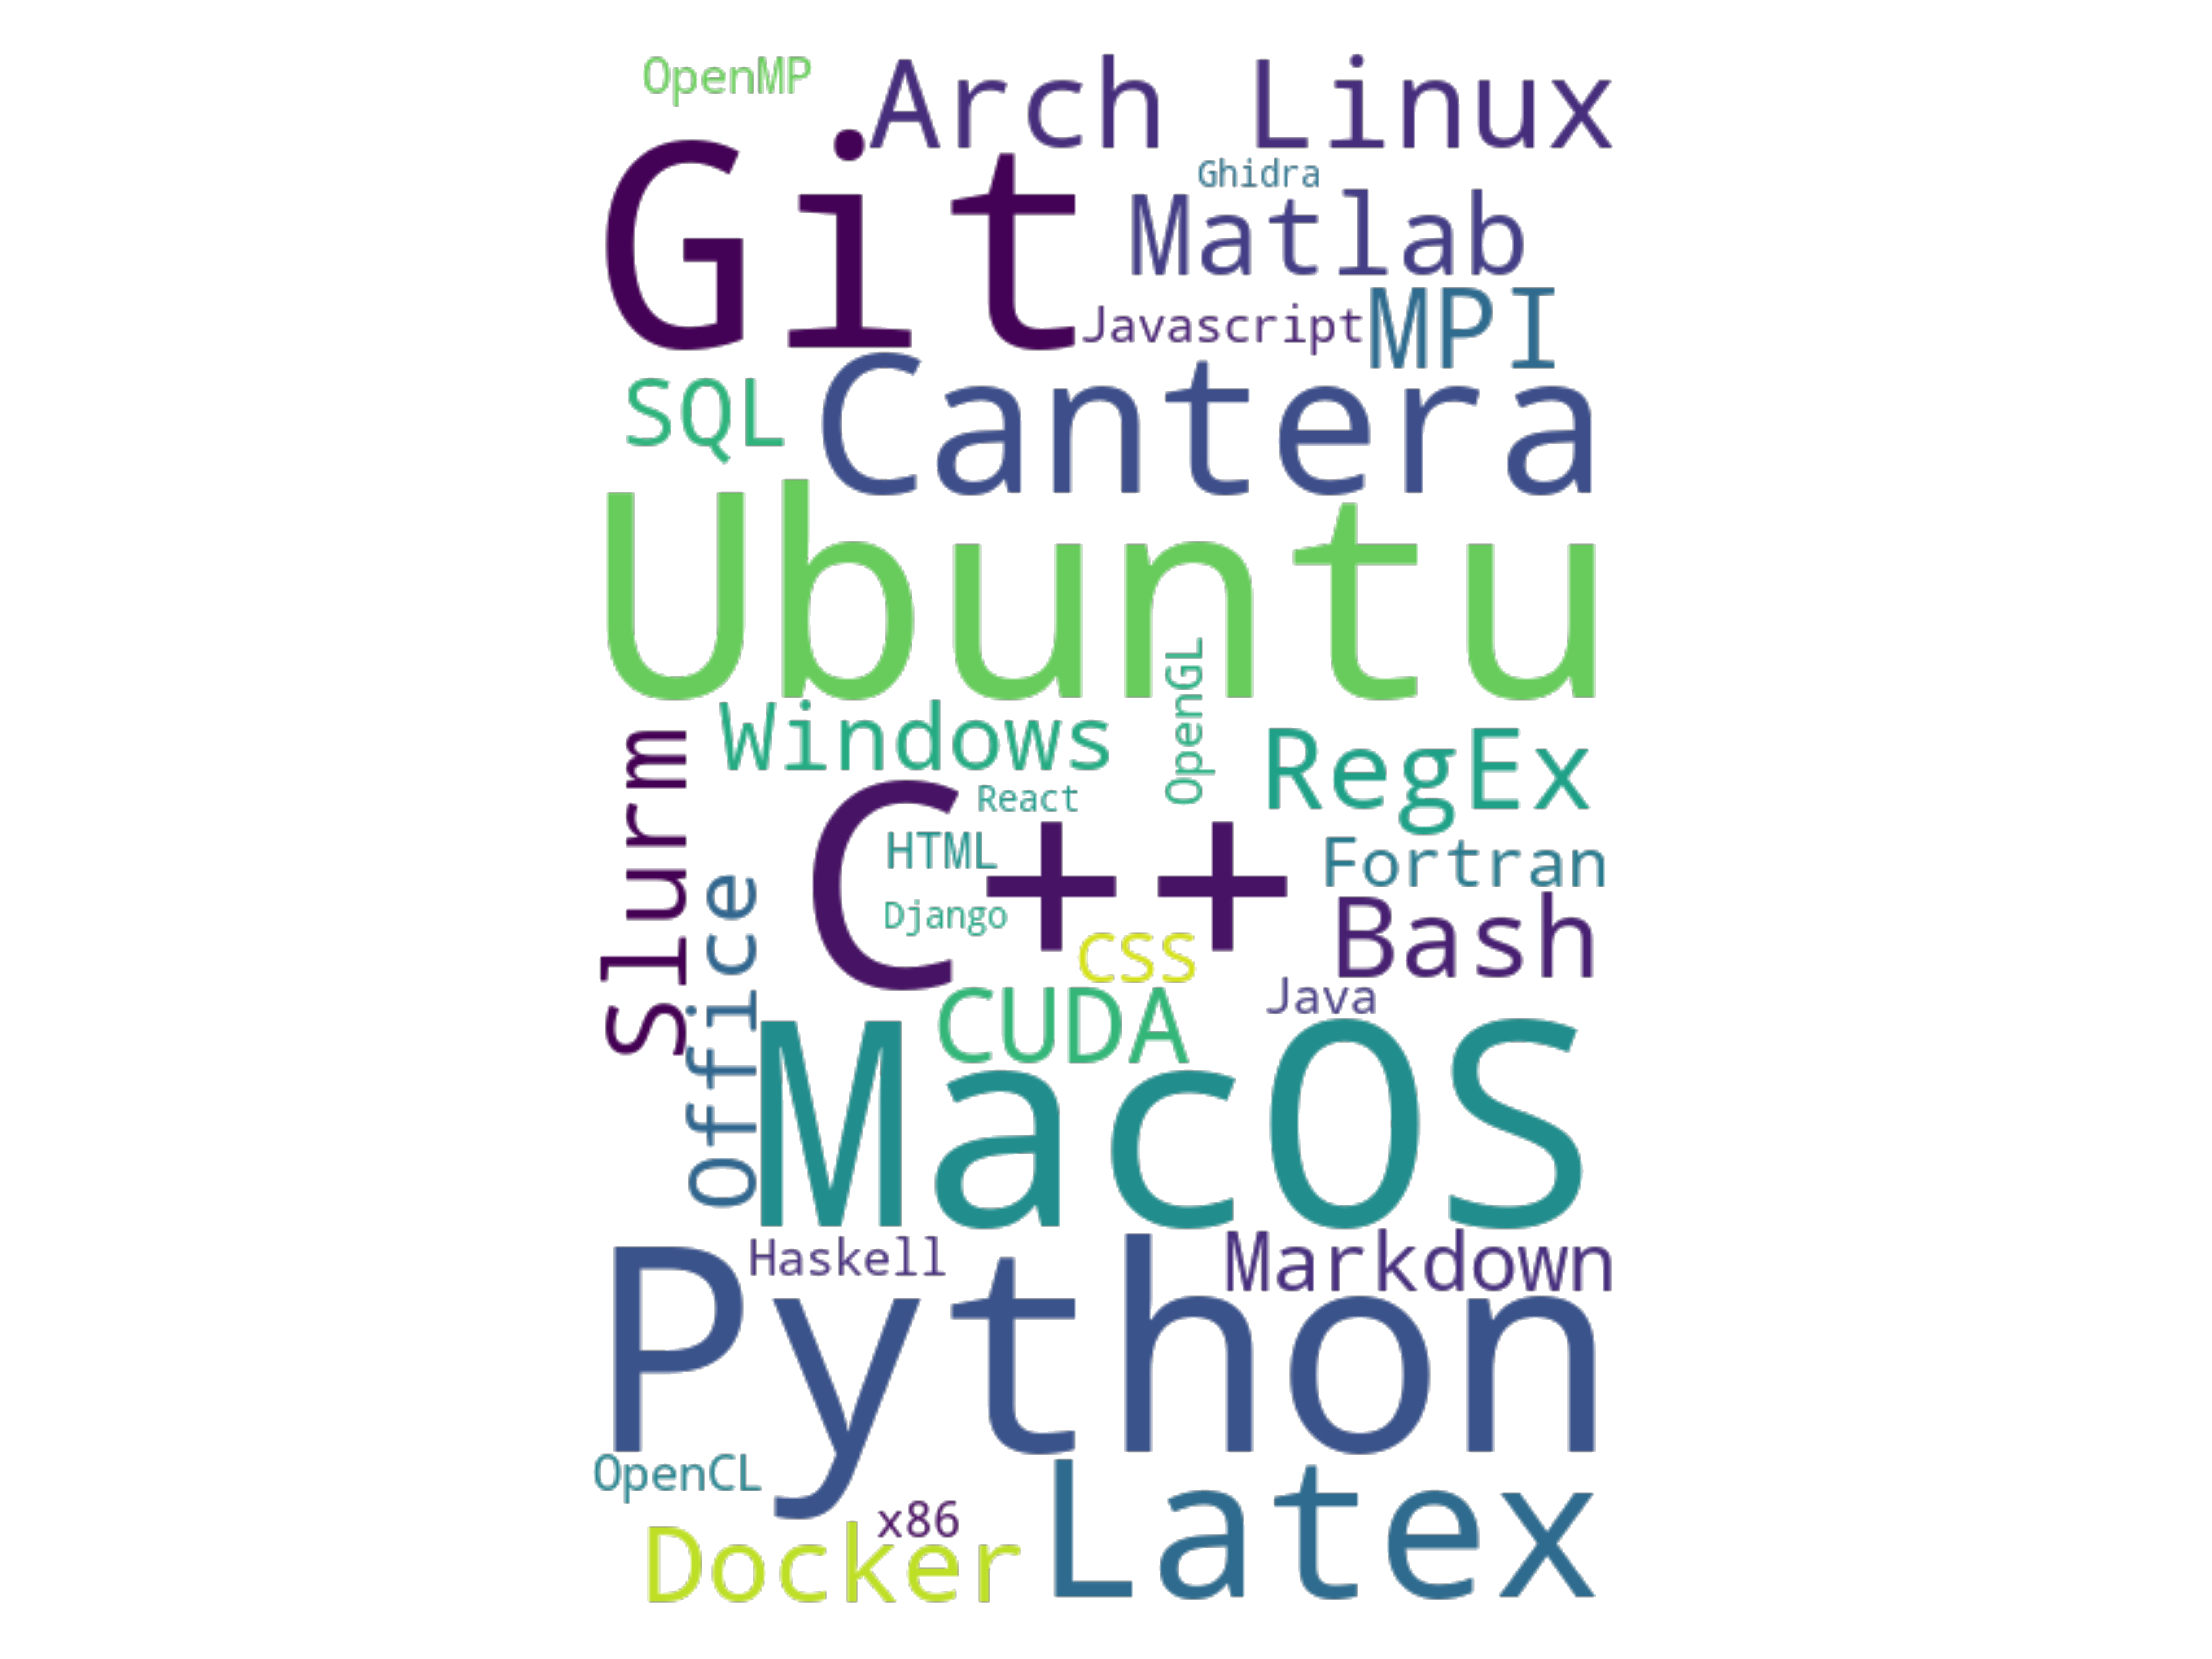
\includegraphics[scale=0.65,trim={4.25cm 0.4cm 4.25cm 0.4cm},clip]{transparent.png}
\end{center}


\section{\faLanguage}{Languages}{cldteal}{1.5cm}
\begin{tabular}{l | l}
\textbf{English} & {\phantom{x}\footnotesize Native} \\
\textbf{French} & \pictofraction{\faCircle}{cldblgry}{3}{black!30}{2}{\tiny} \\
% \textbf{Portuguese} & \pictofraction{\faCircle}{cldgrnbl}{1}{black!30}{4}{\tiny} \\
% \textbf{Japanese} & \pictofraction{\faCircle}{cldprp}{1}{black!30}{4}{\tiny} \\

\end{tabular}

\end{flushleft}

\phantom{turn the page}

\phantom{turn the page}
}
%-----------------------------------------------------------
\switchcolumn

\small
\section{\faGears}{Employment}{cldteal}{7.65cm}

\begin{tabular}{r| p{0.5\textwidth} c}
    \cvevent{Aug 2016--May 2018}{Undergraduate Research Assistant}{Penn State}{Erie PA \color{cldgrnbl}}{\begin{itemize}
        \item Developed software for modeling of piezo-electric power generation in turbulent flow.
    \end{itemize}}\\
    \cvevent{May 2017--Aug 2017}{Test Stand Engineering Intern}{Bell Helicopter}{Fort Worth TX \color{cldblgry}}{
    \begin{itemize}
        \item Developed a troubleshooting guide for repair and maintenance of test stand systems.
    \end{itemize}}\\
    \cvevent{Sept 2018--March 2024}{Graduate Research Assistant}{Oregon State University}{Corvallis OR \color{cldprp}}{\begin{itemize}
        \item Development of a heterogeneous coupled GPU/CPU solver to reduce latency and accelerate simulations of multi-dimensional PDEs.
        \item Open source development within \href{https://cantera.org/}{Cantera} to accelerate chemical kinetics with advanced numerical techniques.
    \end{itemize}} \\
    \cvevent{April 2022--Present}{Software Engineer}{Kairos Power}{Alameda CA \color{cldteal}}{\begin{itemize}
        \item Development and maintenance of a package to automatically generate input files for a \href{https://www.anl.gov/nse/system-analysis-module}{nuclear design code}.
        \item Development of automatic verification software for the core-design team.
        \item Various miscellaneous responsibilities such as database setup, numerical benchmarking, and automated memo generation.
    \end{itemize}}
\end{tabular}

\section{\faFile}{Publications}{cldgrnbl}{7.5cm}

\publication
{The atmospheric evolution of SOA precursor emissions from jet engines when burning sustainable aviation fuel blends with farnesane}
{\textbf{Walker, Anthony S.} Speth, Raymond L. Niemeyer, Kyle E.}
{2024}
{Manuscript in preparation}
{}

\publication
{Extending generalized preconditioning to accelerate simulations of coupled reactor and surface systems}
{\textbf{Walker, Anthony S.} Speth, Raymond L. Niemeyer, Kyle E.}
{2023}
{Manuscript in preparation}
{}

\publication
{Generalized preconditioning for accelerating simulations with large kinetic models}
{\textbf{Walker, Anthony S.} Speth, Raymond L. Niemeyer, Kyle E.}
{2022}
{PROCI: Proceedings of the Combustion Institute,\\https://doi.org/10.1016/j.proci.2022.07.256}
{}
%     ``'', at: \emph{39th International Combustion Symposium} in Vancouver, \textbf{July 2022}.

\publication
{The two-dimensional swept rule applied on heterogeneous architectures.} % Title
{\textbf{Walker, Anthony S.} \& Niemeyer,  Kyle E.} % Authors
{2021} % Year
{MDPI: Mathematical and Computational Applications,\\ https://doi.org/10.3390/mca26030052} % Journal
{} % ADS & arxiv links
\publication
{Applying the swept rule for solving explicit partial differential equations on heterogeneous computing systems} % Title
{Magee, Daniel J \& \textbf{Walker, Anthony S} \& Niemeyer, Kyle E} % Authors
{2020} % Year
{Journal of Supercomputing,\\ https://doi.org/10.1007/s11227-020-03340-9} % Journal
{\color{black}\pgfsetfillopacity{1}} % ADS & arxiv links



% \section{\faCode}{Programming \& Software}{cldblgry}
% \begin{center}
%     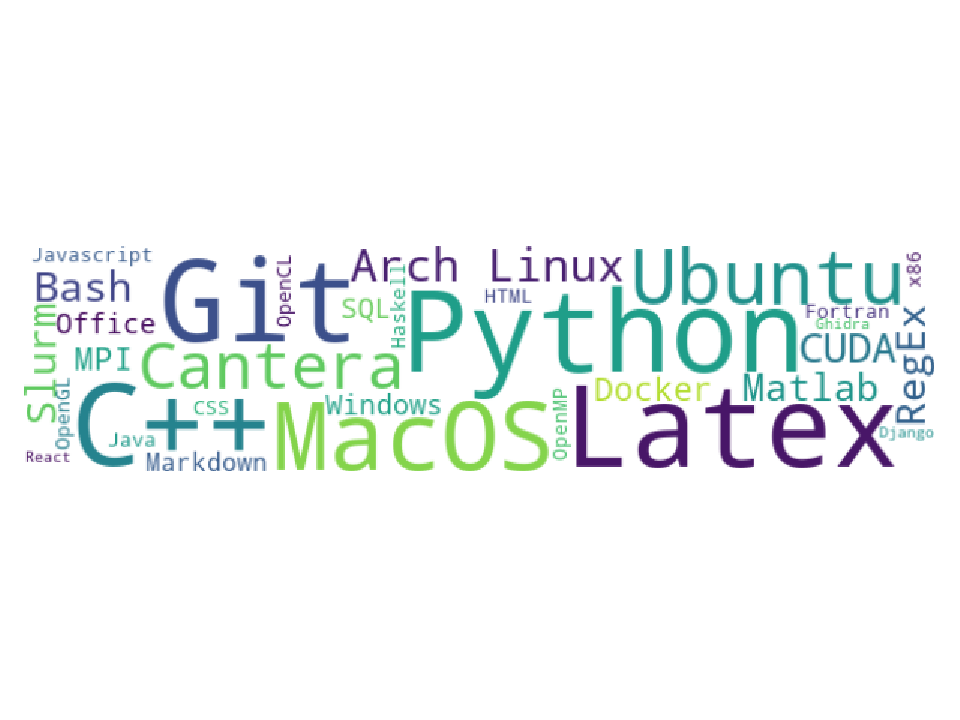
\includegraphics[scale=0.75,trim={0.25cm 4cm 0.25cm 4cm},clip]{CV/cv-cloud.pdf}
% \end{center}



% \begin{minipage}[t]{0.25\textwidth}
% \section*{References}
% \begin{tabular}{l l l}
%     Kyle Niemeyer & Academic Advisor & kyle.niemeyer@oregonstate.edu\\
%     Lambert Fick & Technical Lead   & fick@kairospower.com\\
%     Kaz Teope & Colleague           & 630-205-7543\\
% \end{tabular}
% \end{minipage}\hfill

\vfill{} % Whitespace before final footer

%----------------------------------------------------------------------------------------
%	FINAL FOOTER
%----------------------------------------------------------------------------------------
% \setlength{\parindent}{0pt}
% \begin{minipage}[t]{\rightcolwidth}
% \begin{center}\fontfamily{\sfdefault}\selectfont \color{black!70}
% \icon{\faGears}{cldprp}{} {\small Anthony Walker \icon{\faPhone}{cldblgry}{} 707-337-3595 \icon{\faEnvelopeO}{cldgrnbl}{} \protect\url{walkanth@oregonstate.edu}
% }
% \end{center}
% \end{minipage}

\end{paracol}

\end{document}
